\label{sec:introduccion}

\section{Antecedentes}
	El problema de la calendarización de actividades es ampliamente conocido y estudiado, el mismo tiene sus distintas divisiones, existen problemas de calendarización de actividades, de juntas, de servicios de transporte y de actividades escolares, a lo largo de el siguiente documento nos vamos a enfocar en el último tipo. La calendarización de actividades escolares ha sido ampliamente estudiada por su complejidad particular puesto que se tienen que considerar varias restricciones y distintos recursos.\\
	
	Actualmente hay varios artículos que hablan al respecto, para el presente trabajo tomamos particularmente tres en cuenta:\\
	
	\textbf{Survey on University Timetabling Problem} \\
	
	De este artículo destacamos la explicación de las clasificaciones de problemas de calendarización de actividades universitarias. \\
	
	Categorías de problemas de acuerdo a sus características:
		
		\begin{itemize}
			\item UTTP: Problema de Horarios de Universidades
			en cuyo caso las clases son asignadas de forma semanal y se tienen que asignar materias a las clases dentro de un horario.
			
			\item CTTP: Problema de Horarios por Curso
			Se refiere al problema de las clases impartidas de un curso/materia a la semana en que el problema incluye asignarles salones y profesores a las materias dentro de un horario.
			
			\item LTTP: Problema de horarios por clase
			Se refiere al problema de asignar una sola clase de un curso por día en la universidad sin que se translapen unas con otras.
			
			\item ETTP: Problema de horarios por examinación
			Contiene una gran cantidad de situaciones propias de los demás problemas. La capacidad de los salones y el horario de profesores y alumnos debe ser tomado en cuenta.
			
		\end{itemize}
	\textbf{Modelling constraints in school timetabling using Integer linear programming} \\
	
	En este artículo encontramos mencionado que existe una categoría para los problemas de calendarización de actividades escolares, este se conoce como STTP: School Timetabling Problem. Los problemas de tipo STTP son aquellos que toman el cuenta el caso de preparatorias y secundarias donde se imparte determinado número de clases por día pero durante todo un período escolar es el mismo profesor quien imparte la misma materia en el mismo grupo en dichos días y horarios.  
		
	\textbf{Applying evolutionary computation to the school timetabling problem: The Greek case} \\
	
	De este artículo es interesante resaltar su aproximación al problema. Definen el problema como uno de minimización con penalizaciones, esto significa que para determinar que una solución es buena se deben violar el menor número de restricciones posible.\\
	
	Las restricciones del problema dan paso a las penalizaciones pero hay restricciones escenciales(hard constraints) y resctricciones no escenciales(soft constraints). El artículo indica que las restricciones escenciales son aquellas que deben ser cumplidas en todo momento para que las solución sea considerada viable y como tal deben tener una penalización bastante mayor a las no escenciales de manera que se favorezca a las soluciones viables. Las restricciones no escenciales son aquellas que ayudan a discriminar entre dos soluciones viables aquella que es mejor. De esta manera la función objetivo es una sumatoria entre las penalizaciones de las restricciones escenciales y no escenciales.
	   
\section{Problema de negocio}
	En la Escuela Superior de Cómputo la generación de la estructura educativa requiere de aproximadamente 3 meses, durante este tiempo se pueden realizar cambios en la asignación realizada incluso momentos antes de que aparezcan en el SAES. El tiempo estimado para la asignación manual de horarios equivale a 10 profesores por cada dos días, este proceso lo llevan a cabo los jefes de departamento y presidentes de academia. \\
	
	Con base en lo anterior, la forma en la que se genera la estructura educativa requiere de tiempo excesivo debido a que la asignación se hace de manera manual. Esta solución se considera la mejor desde el punto de vista de los jefes de academia, y depende totalmente de la perspectiva de cada uno de ellos.

\section{Solución}
	A fin de abordar el problema presentado, se propone la utilización de cómputo evolutivo. Es importante recalcar que si bien, puede existir una solución ideal, el espacio de la búsqueda es exponencial en función al número de atributos que utilicemos, por lo tanto encontrar esta solución podría tardar mucho tiempo o incluso podría darse el caso que no se encuentre nunca. \\
	
	Este problema de asignación de horarios está relacionado con la complejidad temporal NP-hard, esto es, el tiempo necesario para llegar a la solución óptima se eleva de manera exponencial de aceurdo al número de variables, esto por el tamaño del espacio de búsqueda. Para el caso de la ESCOM, se cuentan con las variables: espacios (salones-laboratorios), profesores, unidades de aprendizaje, grupos, horarios. Con este conjunto de variables se estudiarán los diferentes algoritmos relacionados a los problemas NP-hard para obtener la función que nos permitirá ofrecer una solución al problema.\\
	
	Debido a la complejidad particular del caso ESCOM en que se tienen alrededor de 200 profesores que son los que se tienen en la nómina, número que puede aumentar o disminuir de acuerdo a las necesidades de la escuela cada semestre, 84 unidades de aprendizaje que son el total de las aprobadas dentro del plan de estudios aunque se pueden o no impartir durante dicho semestre, 14 posibles horarios debido a que en ESCOM ya que casi todas las unidades de aprendizaje duran una hora y media y se imparten 3 días a la semana por lo que se han configurado los horarios en 14 posibles combinaciones de tres sesiones a la semana. Se tienen también al rededor de 36 salones utilizables para impartir clase, finalmente se generan al rededor de 72 grupos al semestre, atacando este problema por fuerza bruta, el total de posibles opciones es aproximadamente 609,638,400 combinaciones lo cuál lo vuelve un espacio de búsqueda demasiado grande como para poder atacarlo de manera tradicional o por fuerza bruta. \\
	
	Como parte de la solución, la primer aproximación será dividir el espacio de búsqueda de acuerdo a las restricciones de ESCOM, en primer lugar los profesores solo imparten un número finito de unidades de aprendizaje al semestre, en segundo lugar los grupos se asocian directamente a un salón, en tercer lugar las unidades de aprendizaje y grupos se dividen por nivel y finalmente los horarios de clase así como los profesores pueden ser matutinos o vespertinos. De esta manera cada particular espacio de búsqueda se reduce a alrededor de 54,600 posibilidades, de esta forma aún es un espacio demasiado grande para métodos tradicionales pero disminuye lo cual aumenta la posibilidad de encontrar una solución viable.\\
	
	Entre las posibles soluciones usuales para este tipo de problemas se propone el uso de algoritmos genéticos sin embargo para este caso en particular la probabilidad de que el algoritmo llegue a la solución óptima es muy baja, podría ser también que la solución final no sea viable, sin mencionar tanto el costo en tiempo como el costo computacional de esto.\\
	
	Finalmente después de analizarlo, y siguiendo las bases de uno de los artículos ya mencionados, se decidió que la mejor aproximación es utilizar programación genética con el operador de mutación, debido a que de esta manera al evaluar la viabilidad de la solución mientras está siendo creada se asegura llegar a una solución viable, que quizás no sea la mejor, pero al crear soluciones viables aseguramos que se resuelva el problema, y la segunda parte del algoritmo se enfoca a evaluar la solución de forma que se pueda definir con base en los criterios definidos por el usuario cual es la mejor solución de entre las propuestas.\\

\section{Objetivos}
	Desarrollar una herramienta que permita generar una o varias opciones de configuración de horarios, tomando en cuenta las restricciones derivadas del análisis del proceso de generación de horarios de la Escuela Superior de Cómputo.
	
	\begin{itemize}
		\item Seleccionar las restricciones a tomar en cuenta para la generación de horarios y definir así el alcance del proyecto.
		
		\item Identificar que técnica meta-heurística debe ser utilizada y adaptar las restricciones disponibles, para el  desarrollo del algoritmo que genera la o las propuestas de horario. 
		
		\item Diseñar la función a optimizar, la cual modela el problema de la generación de propuesta de horario.
	
		\item Desarrollar un sistema que nos permita la visualización de los resultados que arroja el algoritmo, así como la gestión de los datos necesarios que se requieren para llevar a cabo la operación.
		
	\end{itemize}
	

\section{Justificación}
	Para comprender mejor el proceso que la estructura educativa conlleva, nos entrevistamos con el subdirector académico M. en C. Iván Giovanny Mosso García, quien nos explicó los diferentes aspectos aquí expuestos. \\
	
	Con base en la entrevista realizada, concluimos que la ESCOM no cuenta con una herramienta en software que ayude a la generación automatizada de la estructura educativa.  \\
	
	El tiempo requerido es excesivo, los involucrados ven reducido el tiempo que pueden invertir en otras actividades. Un problema aún mayor radica en que la propuesta de la estructura educativa debe ser aprobada por la DAE, después de lo cual puede ser
	que se presenten cambios y esto implica un incremento de tiempo y esfuerzo del personal de la ESCOM en dicho proceso, mismos que aún con toda la experiencia que tienen pueden llegar a cometer errores debido a la complejidad del proceso.  \\
	
	De acuerdo a lo anterior la importancia del proyecto radica, esencialmente, en la asignación de recursos y tiempo que representaría dentro del proceso de generación de horarios, ya que se plantea que el proceso concluya con opciones viables de horarios de acuerdo a las características que se tienen en la escuela debido a que no solo se tiene que generar una propuesta de los horarios y esto no implica únicamente agrupar clases en bloques sino que el problema escala hasta la asociación de grupos, profesores, materias, salones, laboratorios y horas mismos que en conjunto son denominados horarios.
	
\section{Estado del arte}

	\begin{itemize}
		\item \textbf{Software comercial} \\ \\
		
		
			\resizebox*{15cm}{8cm}{
			\begin{tabular}{|c |c |l|}
				\hline
				Nombre & Compañía & Descripción\\
				\hline
				GHC & Peñalara & Gestión completa de horarios escolares y universitarios.\\
				&&Presentes en 25 países, en más de 3500 centros de enseñanza.\\
				&&Aplicación de paga.\\
				\hline
				UnitsExpress & Units Grubbers \& Petters & Aplicación de escritorio.\\
				&&Generación de horarios de acuerdo a los criterios pedagógicos que se seleccionen.\\
				&&Posibilidad de visualización y cambios del resultado.\\
				&&Aplicación de paga. \\
				\hline
				Timetable & Timetable web & Aplicación en línea. \\
				&&Aplicación de paga. \\
				&&Funciona en cualquier sistema operativo. \\
				&&Velocidad de respuesta. \\
				&&Inserción de restricciones. \\
				&&Impresión en pdf. \\
				\hline
				HorarioFacil & Horário Fácil & Aplicación en línea. \\
				&&Aplicación de paga.\\
				&&Proceso de 6 pasos.\\
				&&Impresión en pdf.\\
				&&Licencia por tiempo. \\	
				\hline
				Wisetimetable & Wisetimetable & Aplicación de escritorio o móvil. \\
				&&Distintos lenguajes \\
				&&Posibilidad de trabajar manualmente, generar automáticamente o mixto. \\
				\hline
		\end{tabular}}\\ \\

		\item \textbf{Tesis} \\ \\
		
		\begin{figure}[htbp!]
			\begin{center}
				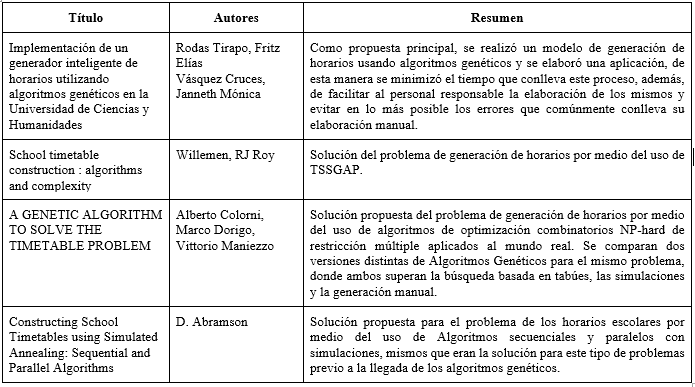
\includegraphics[width=1.05\textwidth]{images/entornoTT/estadoArteTesis.png}
				
			\end{center}
		\end{figure}
	\end{itemize}
		
		%\begin{tabulary}{10 cm}{|J|J|J|}
%			\hline
%			Título & Autores & Resúmen\\
%			\hline
%			Implementación de un generador inteligente de horarios utilizando algoritmos genéticos en la Universidad de Ciencias y Humanidades & Rodas Tirapo, Fritz Elías	Vásquez Cruces, Janneth Mónica
%			 & Como propuesta principal, se realizó un modelo de generación de horarios usando algoritmos genéticos y se elaboró una aplicación, de esta manera se minimizó el tiempo que conlleva este proceso, además, de facilitar al personal responsable la elaboración de los mismos y evitar en lo más posible los errores que comúnmente conlleva su elaboración manual. \\
%		
%			\hline
%			School timetable construction : algorithms and complexity & Willemen, RJ Roy & Solución del problema de generación de horarios por medio del uso de TSSGAP.\\
%		
%			\hline
%			A GENETIC ALGORITHM TO SOLVE THE TIMETABLE PROBLEM & Alberto Colorni, Marco Dorigo, Vittorio Maniezzo & Solución propuesta del problema de generación de horarios por medio del uso de algoritmos de optimización combinatorios NP-hard de restricción múltiple aplicados al mundo real. Se comparan dos versiones distintas de Algoritmos Genéticos para el mismo problema, donde ambos superan la búsqueda basada en tabúes, las simulaciones y la generación manual. \\
%			
%			\hline
%			Constructing School Timetables using Simulated Annealing: Sequential and Parallel Algorithms & D. Abramson  & Solución propuesta para el problema de los horarios escolares por medio del uso de Algoritmos secuenciales y paralelos con simulaciones, mismos que eran la solución para este tipo de problemas previo a la llegada de los algoritmos genéticos. \\
%			
%			\hline
	%\end{tabulary}
	
	


	
	
	
	